
\documentclass[a4paper,12pt]{article}

\usepackage{url}
\usepackage{graphicx}

\newcommand{\id}[1]{{\scshape\small #1}}
\newcommand{\psim}{\id{Peersim}}

\title{PeerSim HOWTO 2: build a topology generator}

\author{Gian Paolo Jesi (jesi@cs.unibo.it)}
\date{November 16, 2005}

\begin{document}

\maketitle

\section{Introduction}

\textbf{NOTE: This tutorial revision covers \psim~release 1.0
  topics.}\\

This tutorial teaches you how to build from scratch a new \psim~
( \psim~ project page: \url{http://sourceforge.net/projects/peersim}
) topology generator. In order to understand this tutorial, the reader
is encouraged to start reading the first \psim~ tutorial 
(\url{http://peersim. sourceforge.net/peersim_HOWTO.html}) 
to have an idea of the basic concepts that will not be discussed any
further in this document. 

The aim of this tutorial is to be as practical as possible; the goal
is to give the reader ideas about technical or intermediate level
features of \psim~ and to encourage him/her to experiment further.
The full source code discussed in this document is available via CVS
at \psim~ project page in the \emph{peersim.example.hot} class package.


\section{What is a topology?}

The network abstraction in \psim~ is a (sometimes huge) array of
\emph{Node} structures (interfaces); because of the size of the network
and to overcome scalability problems, usually in large P2P networks
each node knows about the existence of a very small subset of other
nodes (e.g., order of $\log(N)$ where $N$ is the whole network size). Thus
each node has a short list of other node references, usually called
``neighbors'', build accordingly to some kind of strategy
or rule. 

Thus, we can say that a topology is how nodes are arranged (linked)
together and clearly this depends upon the particular chosen rule.
Examples of topology are the following (not exhaustive at all): 

\begin{itemize}
\item random graphs 
\item Watts-Strogatz model graph 
\item star model 
\item ring model 
\item lattice model 
\item ...
\end{itemize}

\subsection{Which rule to choose?}
\label{sec:rule}

In this document, we have chosen to code a particular topology generator
to build Internet-like tree topologies. The building process is based
on the \emph{preferential attachment} approach. The rule applied is
quite simple and takes into account geometric and network constraints
to better mimic real world network. The preferential attachment choice
can be affected by a parameter ($ \alpha $) that amplifies or reduces the
geometric location influence in favor of the path distance. 

The rule strategy is the following: we consider a square unit region
$D$, then we start with node $x(0)$ chosen at random and we set $W(x(0))
= 0$ (it i

s the root node). For each i with $i = 1...n-1$ we choose a
new node $x(i)$ in the region $D$ and we connect it to an \textbf{early
inserted} node $x(j)$ that minimize the following formula:

\begin{center}
$W(x(j)) + \alpha \cdot dist(x(i), x(j))$ with 0 $\leq$ j $<$ i
\end{center}

where: 

\begin{itemize}
\item $W(x(j))$ is the distance in terms of hops (the path distance from node
$x(j)$ to the root node); 
\item $dist(...)$ is the usual Euclidean distance; 
\item $ \alpha $ is a weight parameter that can minimize or maximize 
the geometric distance influence;
 
\end{itemize}

After having chosen a node $x(j)$, we set $W(x(i)) = W(x(j))+1$ . At
the end we obtain a tree rooted in $x(0)$. This topology implies that
every node (except the root) has an out-degree of exactly one link.

%We have extended this model to improve robustness allowing every node
%to have exactly $d$ outbound neighbors instead of only one. This means
%that, at the time of joining the network, each node should have at
%least $d$ candidates to be selected as neighbors. To achieve this property,
%as a first step we select at random exactly $d$ root nodes and we connect
%them together in a ring fashion (a doubly linked list). In this way
%each ordinary node has at least $d$ nodes (the $d$ roots) to choose from
%in order to select its neighbors. In other words, each node has to
%select the best $d$ nodes that minimize the function above. 

To get further details about this model, we suggest the following
readings:

\begin{enumerate}

\item ``Heuristically Optimized Trade-offs: A New Paradigm for Power
Laws in the Internet'' \\
(\url{http://cgi.di.uoa.gr/~elias/publications/paper-fkp02.pdf} )

\item  ``Degree distributions
of the FKP network model'' \\
(\url{http://research.microsoft.com/~jchayes/Papers/FKPdgrees.pdf}) 

\item ``On Power-Law
Relationships of the Internet Topology''\\
(\url{http://www.cs.ucr.edu/~michalis/CAMERA.ps})

\end{enumerate}

The model should generate a topology that exhibits a power-law bound
on the in-degree sequence of nodes; but, as stated in the second
previously listed paper, this power-law prediction is not true. In fact
this preferential attachment model does not generate always such an
in-degree sequence 
distribution, but for some parameter values it shows a power-law like
behaviour. 

\section{What we need to code}
\label{s:coding}

Our aim is to write a standard \psim~component able to produce the
desired topology according to the $\alpha$ parameter. Apart from the
$\alpha$ parameter, the algorithm relies also on how the nodes are
distributed in the squared area. We choose to initialize their
2d-coordinates using a uniformly random distribution.

We are not interested
in building the topology in a set of steps over time: we want
something like a topology initializer that arranges the wiring from scratch in
one step.

In order to build the desired topology, we need to extend or implement
the following classes/interfaces:  

\begin{itemize}

\item the \emph{Protocol} class: the protocol itself does nothing; we
  need a place to store some informations, such as the coordinates.
The reader can think to this class as ``glue code''.
 
\item the \emph{Control} interface: we need several \emph{Control}
  implementing classes in order to perform the following task:

\begin{itemize}

\item Initialize the 2d-coordinates for each node and select an
  initial root node.

\item An observer is needed to print the topology to a file (e.g., to
  visualize the generated graph using GnuPlot).

\item An observer can be used to collect statistics about the
  in-degree distribution.

\item Another observer can test the topology robustness to random node
  failures.

\end{itemize}

\item A class dedicated to the actual node wiring process according to
  the rules described in Section~\ref{sec:rule}. It can be considered
  as a \emph{factory} component.

\end{itemize}

As we will see in next sections, some of the classes we intend to code
are not needed. \psim~standard components can be used instead. It is
important to decouple carefully all the tasks we intend to accomplish in
order to figure out if there are ``common patterns'' that are already
available and ready to use.


\section{Code writing}

\subsection{Protocol class}

As we stated so far, the protocol code is minimal:

\footnotesize
\begin{verbatim}
package example.hot;

import peersim.core.Protocol;

public class InetCoordinates implements Protocol {

    // ------------------------------------------------------------------------
    // Fields
    // ------------------------------------------------------------------------
    /** 2d coordinates components. */
    private double x, y;

    // ------------------------------------------------------------------------
    // Constructor
    // ------------------------------------------------------------------------
    public InetCoordinates(String prefix) {
        /* Un-initialized coordinates defaults to -1. */
        x = y = -1;
    }

    public Object clone() {
        InetCoordinates inp = null;
        try {
            inp = (InetCoordinates) super.clone();
        } catch (CloneNotSupportedException e) {
        } // never happens
        return inp;
    }

    public double getX() {
        return x;
    }

    public void setX(double x) {
        this.x = x;
    }

    public double getY() {
        return y;
    }

    public void setY(double y) {
        this.y = y;
    }

}
\end{verbatim}
\normalsize

The actual ``who knows whom'' relation (the topology) container is decoupled
from this class. Any standard \psim~component implementing the
\emph{Linkable} interface can be used (see the configuration file in
Section~\ref{s:experiments}). 

The class is basically a structure encapsulated in an
object to hold the $x$ and $y$ coordinate components. Another solution
could be to define a specialized sub-class of 
\emph{peersim.core.GeneralNode} in which the coordinate be stored
and then use \emph{peersim.core.IdleProtocol} to handle the nodes
``who knows whom'' relations. Both the approaches are identical in
practice, it is just a developer choice. The reader can implement this
second suggestion just for exercise.

The \emph{clone()} method must be redefined according to the
\emph{Protocol} class contract. It does not have to do much: there
are only primitive types that are cloned by default.

The coordinates components are not public and can be accessed by their
getter/setter methods.

\subsection{Initialization class}
\label{s:init}

\footnotesize
\begin{verbatim}
package example.hot;

import peersim.config.Configuration;
import peersim.core.CommonState;
import peersim.core.Control;
import peersim.core.Network;
import peersim.core.Node;

public class InetInitializer implements Control {
    // ------------------------------------------------------------------------
    // Parameters
    // ------------------------------------------------------------------------
    private static final String PAR_PROT = "protocol";

    // ------------------------------------------------------------------------
    // Fields
    // ------------------------------------------------------------------------
    /** Protocol identifier, obtained from config property {@link #PAR_PROT}. */
    private static int pid;

    // ------------------------------------------------------------------------
    // Constructor
    // ------------------------------------------------------------------------
    public InetInitializer(String prefix) {
        pid = Configuration.getPid(prefix + "." + PAR_PROT);
    }

    // ------------------------------------------------------------------------
    // Methods
    // ------------------------------------------------------------------------
    /**
     * Initialize the node coordinates. The first node in the {@link Network} is
     * the root node by default and it is located in the middle (the center of
     * the square) of the surface area.
     */
    public boolean execute() {
        // Set the root: the index 0 node by default.
        Node n = Network.get(0);
        InetCoordinates prot = (InetCoordinates) n
                .getProtocol(pid);
        prot.setX(0.5);
        prot.setY(0.5);

        // Set coordinates x,y
        for (int i = 1; i < Network.size(); i++) {
            n = Network.get(i);
            prot = (InetCoordinates) n.getProtocol(pid);
            prot.setX(CommonState.r.nextDouble());
            prot.setY(CommonState.r.nextDouble());
        }
        return false;
    }

}
\end{verbatim}
\normalsize

The initialization class has to implement the \emph{Control} interface
and its only method: \emph{execute()}. 
The constructor reads the only parameter (\texttt{protocol}) from 
the configuration
file. It declares the protocol holding the coordinates.

The class is very simple, it
has to generate uniformly random numbers for each node coordinate
components ($x$ and $y$). The only exception is the root node that, by
default, is the index 0 node. Its coordinate is forced to be $(0.5,
0.5)$. This particular choice is to generate nice looking graphs when
it is time to plot them.

To generate random number, the static field \texttt{r} of
\emph{CommonState} is used.

\subsection{The factory class}
\label{s:factory}

The factory class uses the features of a standard \psim~component:
\emph{peersim.dynamics.WireGraph} (it is a \emph{Control}
instance). The overlay is wired using the 
\emph{Graph} API methods; the wiring logic has to be in the
\emph{wire()} method that is called by the superclass.

The class has to read from the configuration file both the $\alpha$
value parameter (\texttt{alpha} in the config file) and the coordinate
container protocol identifier (\texttt{coord\_protocol} in the config
file). This
is done in the class constructor. The other parameter, \texttt{protocol}
is inherited by the superclass: it is the \emph{Linkable}
implementing protocol identifier.

The \emph{wire()} method contains the wiring rules described in
Section~\ref{sec:rule}.

To keep track of the hop distances, a network sized integer array is
used. Each index $i$ slot value corresponds to the $node_{i}$ hop distance from the
root.

By default, the wiring process considers the index 0 node as the root.

A static utility method, \emph{distance()}, gives the Euclidean
distance between two nodes.


\footnotesize
\begin{verbatim}
package example.hot;

import peersim.config.Configuration;
import peersim.core.Linkable;
import peersim.core.Network;
import peersim.core.Node;
import peersim.dynamics.WireGraph;
import peersim.graph.Graph;

public class WireInetTopology extends WireGraph {
    // ------------------------------------------------------------------------
    // Parameters
    // ------------------------------------------------------------------------
    private static final String PAR_ALPHA = "alpha";

    private static final String PAR_COORDINATES_PROT = "coord_protocol";

    // --------------------------------------------------------------------------
    // Fields
    // --------------------------------------------------------------------------
    /* A parameter that affects the distance importance. */
    private final double alpha;

    /** Coordinate protocol pid. */
    private final int coordPid;

    // --------------------------------------------------------------------------
    // Initialization
    // --------------------------------------------------------------------------
    public WireInetTopology(String prefix) {
        super(prefix);
        alpha = Configuration.getDouble(prefix + "." + PAR_ALPHA, 0.5);
        coordPid = Configuration.getPid(prefix + "." + PAR_COORDINATES_PROT);
    }

    /**
     * Performs the actual wiring. 
     * @param g
     *            a {@link peersim.graph.Graph} interface object to work on.
     */
    public void wire(Graph g) {
        /** Contains the distance in hops from the root node for each node. */
        int[] hops = new int[Network.size()];
        // connect all the nodes other than roots
        for (int i = 1; i < Network.size(); ++i) {
            Node n = (Node) g.getNode(i);

            // Look for a suitable parent node between those allready part of
            // the overlay topology: alias FIND THE MINIMUM!
            // Node candidate = null;
            int candidate_index = 0;
            double min = Double.POSITIVE_INFINITY;
            for (int j = 0; j < i; j++) {
                Node parent = (Node) g.getNode(j);
                double jHopDistance = hops[j];

                double value = jHopDistance
                        + (alpha * distance(n, parent, coordPid));
                if (value < min) {
                    // candidate = parent; // best parent node to connect to
                    min = value;
                    candidate_index = j;
                }
            }

            hops[i] = hops[candidate_index] + 1;
            g.setEdge(i, candidate_index);
        }
    }

    private static double distance(Node new_node, Node old_node, int coordPid) {
        double x1 = ((InetCoordinates) new_node.getProtocol(coordPid))
                .getX();
        double x2 = ((InetCoordinates) old_node.getProtocol(coordPid))
                .getX();
        double y1 = ((InetCoordinates) new_node.getProtocol(coordPid))
                .getY();
        double y2 = ((InetCoordinates) old_node.getProtocol(coordPid))
                .getY();
        if (x1 == -1 | x2 == -1 | y1 == -1 | y2 == -1)
            throw new RuntimeException(
                    "Found un-initialized coordinate. Use e.g.,\
                    InetInitializer class in the config file.");
        return Math.sqrt((x1 - x2) * (x1 - x2) + (y1 - y2) * (y1 - y2));
    }
}
\end{verbatim}
\normalsize
     
\subsection{The observers}
\label{s:observers}

Some of the observer tasks depicted in Section~\ref{s:coding} can be performed
by standard \psim~components available in the distribution. 

For example, to compute statistics regarding the degree distribution, the user can
use the \emph{peersim.reports.DegreeStats} object. To test the network
robustness, \emph{RandRemoval} can be used: it kills nodes randomly
and prints statistics about the number of generated clusters and their
size.\\

However, to dump the topology to a file in a plottable form, we still
need to write our observer: \emph{InetObserver} implementing the \emph{Control}
interface and the corresponding 
\emph{execute()} method. To ease even further our job, we decided to
not implement directly the \emph{Control} interface, but to extend
\emph{persim.reports.GraphObserver}. This template class gives us a
graph API to interact with the protocol to be inspected.

The constructor takes care of reading the parameters from the
configuration file. The \texttt{protocol} parameter refers to the
protocol identifier holding the ``who knows whom'' relation (it is a
\emph{Linkable} protocol). It is inherited by the superclass.

The other parameters, \texttt{coord\_protocol} and \texttt{file\_base},
correspond respectively to the coordinate container protocol
identifier and to the filename base used. 
The final filename generated by
the program is: 

\begin{center}
$<$file\_base$>$ + \%08d + .dat 
\end{center}

The number in the middle of the filename keeps track of the current
cycle number; 8 digits are available as a cycle counter. 
This is due to the fact that, as any control object, the
observer can run at every cycle and in this case a
different file has to be generated at each time. 

\footnotesize
\begin{verbatim}
package example.hot;

import java.io.FileOutputStream;
import java.io.IOException;
import java.io.PrintStream;

import peersim.config.Configuration;
import peersim.core.Node;
import peersim.graph.Graph;
import peersim.reports.GraphObserver;
import peersim.util.FileNameGenerator;

public class InetObserver extends GraphObserver {
    // ------------------------------------------------------------------------
    // Parameters
    // ------------------------------------------------------------------------
    private static final String PAR_FILENAME_BASE = "file_base";

    private static final String PAR_COORDINATES_PROT = "coord_protocol";

    // ------------------------------------------------------------------------
    // Fields
    // ------------------------------------------------------------------------

    private final String graph_filename;

    private final FileNameGenerator fng;

    private final int coordPid;

    // ------------------------------------------------------------------------
    // Constructor
    // ------------------------------------------------------------------------
    public InetObserver(String prefix) {
        super(prefix);
        coordPid = Configuration.getPid(prefix + "." + PAR_COORDINATES_PROT);
        graph_filename = Configuration.getString(prefix + "."
                + PAR_FILENAME_BASE, "graph_dump");
        fng = new FileNameGenerator(graph_filename, ".dat");
    }

    // Control interface method.
    public boolean execute() {
        try {
            updateGraph();

            System.out.print(name + ": ");

            // initialize output streams
            String fname = fng.nextCounterName();
            FileOutputStream fos = new FileOutputStream(fname);
            System.out.println("Writing to file " + fname);
            PrintStream pstr = new PrintStream(fos);

            // dump topology:
            graphToFile(g, pstr, coordPid);

            fos.close();
        } catch (IOException e) {
            throw new RuntimeException(e);
        }

        return false;
    }

    private static void graphToFile(Graph g, PrintStream ps, int coordPid) {
        for (int i = 1; i < g.size(); i++) {
            Node current = (Node) g.getNode(i);
            double x_to = ((InetCoordinates) current
                    .getProtocol(coordPid)).getX();
            double y_to = ((InetCoordinates) current
                    .getProtocol(coordPid)).getY();
            for (int index : g.getNeighbours(i)) {
                Node n = (Node) g.getNode(index);
                double x_from = ((InetCoordinates) n
                        .getProtocol(coordPid)).getX();
                double y_from = ((InetCoordinates) n
                        .getProtocol(coordPid)).getY();
                ps.println(x_from + " " + y_from);
                ps.println(x_to + " " + y_to);
                ps.println();
            }
        }
    }
}
\end{verbatim}
\normalsize

In the \emph{execute()} method we MUST call \emph{updateGraph()} (a
\emph{GraphObserver} protected method) in order to check if some
change has occurred on the actual graph. 
The scope of this mechanism is to save the time of constructing the
graph if many observers are run on the same graph. Time savings can be very
significant if the undirected version of the same graph is observed by
many observers.

In addition, note that in \emph{execute()} method the IO library functions
used may throw some exceptions. In case of troubles, any kind of
exception is catch-ed, but a runtime exception is thrown to stop the
process. 

The static utility method \emph{graphToFile()} writes to disk the
actual topology. The idea is simple: for each node
$n$, the $x$ and $y$ coordinates are collected and then for each
neighbor $i$ of node $n$ the coordinates are written in the following
format: 

\footnotesize
\begin{verbatim}
 n.neighbor(i).x n.neighbor(i).y \newline
 n.x n.y \newline
 \newline}
\end{verbatim}
\normalsize 

The particular line triplet formatting order suits the gluplot needs. 
Please note that the for loop starts from index $1$, not from $0$;
this is due to the fact that node 0 is the root and has no out-bound
connections.

\section{Experiments}
\label{s:experiments}

In order to make the model run, a proper \psim~configuration file is 
needed. The one presented in the following lines may suits the reader needs:

\footnotesize
\begin{verbatim}
# Complex Network file:
#random.seed 1234567890
simulation.cycles 1

network.size 10000

protocol.link IdleProtocol

protocol.coord example.hot.InetCoordinates

init.0 example.hot.InetInitializer
init.0.protocol coord

init.1 example.hot.WireInetTopology
init.1.protocol link #the linkable to be wired
init.1.coord_protocol coord
init.1.alpha 4

control.io example.hot.InetObserver
control.io.protocol link
control.io.coord_protocol coord
control.io.file_base graph

control.degree DegreeStats
control.degree.protocol link
control.degree.undir
control.degree.method freq

include.control io degree
\end{verbatim}
\normalsize

It produces a 10000 node overlay network with the parameters listed in 
the \texttt{init.0} section.

The presented figures show the produced topology and highlight the 
parameter $\alpha$ importance. In fact, it affects the clustering behavior of 
the system and it is tightly correlated to the size of the network. If 
$\alpha$ is lower than $\sqrt{netsize}$, the topology becomes more and more 
clustered (as show in the first two figures); with extremely low $\alpha$, 
the topology becomes a star. On the other end, if $\alpha$ is grater than 
$\sqrt{netsize}$, the topology tends to be random and not clustered at all 
(the second row of images). For deeper details, please consult the previously
listed papers.

As stated in Section~\ref{s:observers}, the \emph{DegreeStats} standard
component can be used to collect degree statistics. However, it should 
be used carefully. By default in \psim,
the ``degree'' is the out-bound degree, while we are interested in the
in-degree. This holds in directed graphs; if the graph is undirected,
the degree is the sum of the out-bound and in-bound degree. So, how
can we inspect the in-degree? The idea is very simple. First we need
to consider the graph as \textbf{undirected} (\texttt{undir}
parameter) and we choose the frequency statistics (\texttt{freq}
parameter) in order to produce our plots. The observer will
print something like:

\footnotesize
\begin{verbatim}
1 9838
2 38
3 19
4 14
5 7
6 7
7 7
8 4
9 3
10 3
11 1
12 5
...
...
543 1
566 1
620 1
653 1
2153 1
\end{verbatim}
\normalsize

The first column corresponds to the degree, while the second to the
number of nodes having that degree. We know for sure that for each node, apart from the
root, there is only one out-bound link. Thus to extract the in-degree
we simply need to subtract 1 from the first column items.

The values shown previously, have been generated with $\alpha = 4$. 

\begin{figure}[tb!]
\begin{center}
\includegraphics[scale=0.6]{pic_alfa01.eps}
\end{center}
\caption{Topology with $\alpha$ 0.1: a star topology.\label{t01figure}}
\end{figure}


The degree distribution related to the generated star topology 
(Figure~\ref{t01figure}) is not 
shown (it is simply a straight line).
Clearly the plots show that there is not any evidence about in-degree 
power-law distribution; only in the case of $\alpha = 4$, the corresponding 
plot exhibits a power-law like behavior at least for a subset of the nodes, 
but this is very different from what first listed paper was talking about.

\begin{figure}[tb!]
\begin{center}
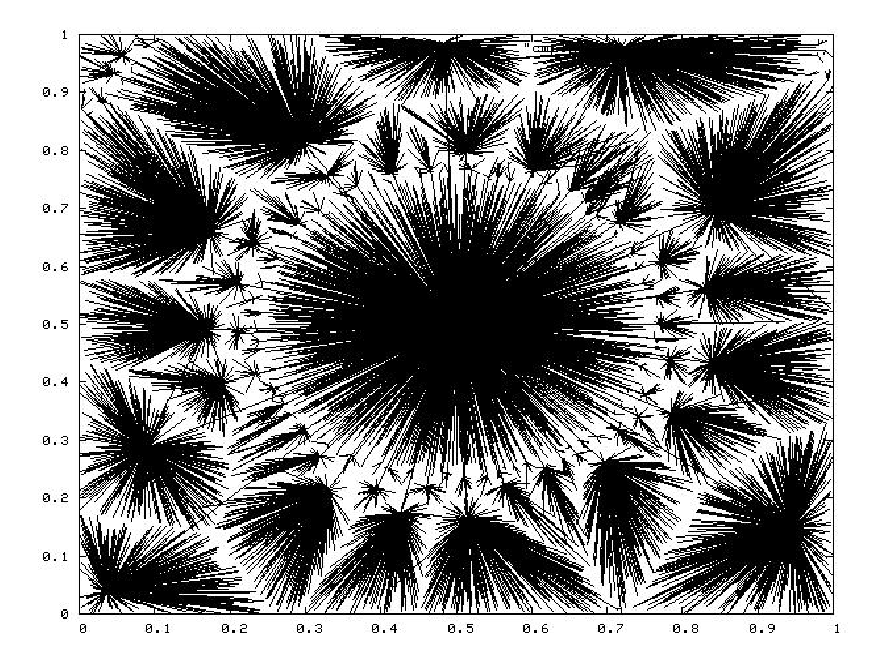
\includegraphics[scale=0.6]{pic_alfa4.eps}
\end{center}
\caption{Topology with $\alpha$ 4\label{t4figure}}
\end{figure}

\begin{figure}[tb!]
\begin{center}
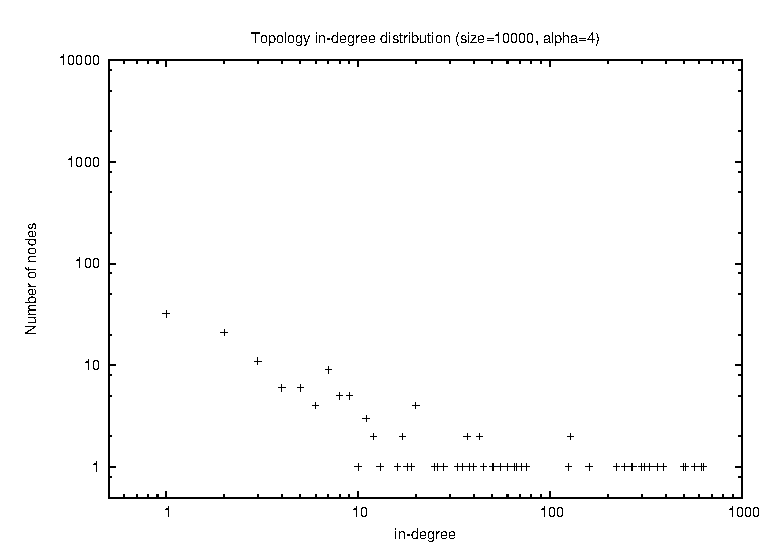
\includegraphics[scale=0.6]{picdegree_alfa4.eps}
\end{center}
\caption{In-degree distribution with $\alpha$ 4 \label{d4figure}}
\end{figure}

\begin{figure}[tb!]
\begin{center}
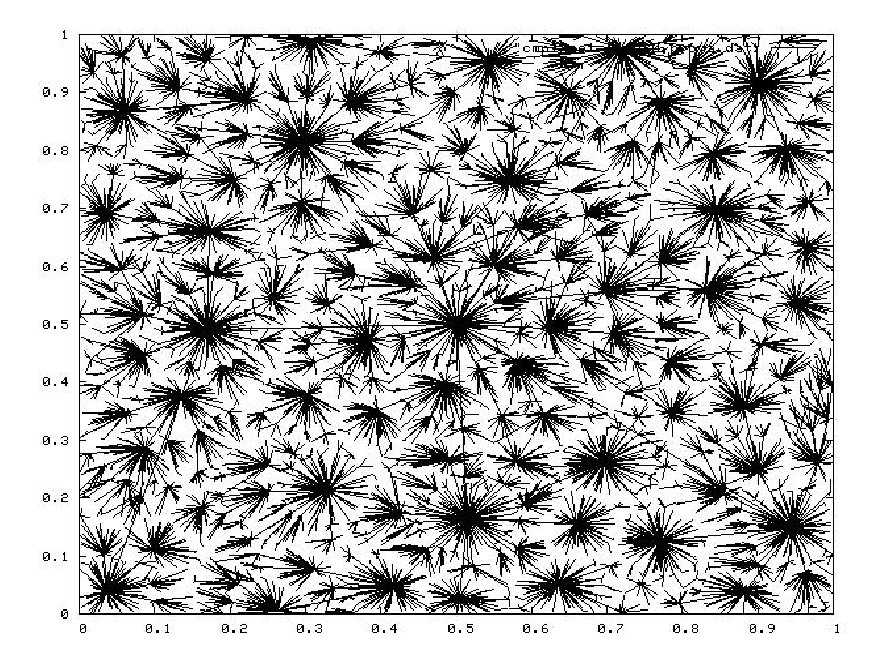
\includegraphics[scale=0.6]{pic_alfa20.eps}
\end{center}
\caption{Topology with $\alpha$ 20\label{t20figure}}
\end{figure}

\begin{figure}[tb!]
\begin{center}
\includegraphics[scale=0.6]{picdegree_alfa20.eps}
\end{center}
\caption{In-degree distribution with $\alpha$ 20 \label{d20figure}}
\end{figure}

\begin{figure}[tb!]
\begin{center}
\includegraphics[scale=0.6]{pic_alfa100.eps}
\end{center}
\caption{Topology with $\alpha$ 100\label{t100figure}}
\end{figure}

\begin{figure}[tb!]
\begin{center}
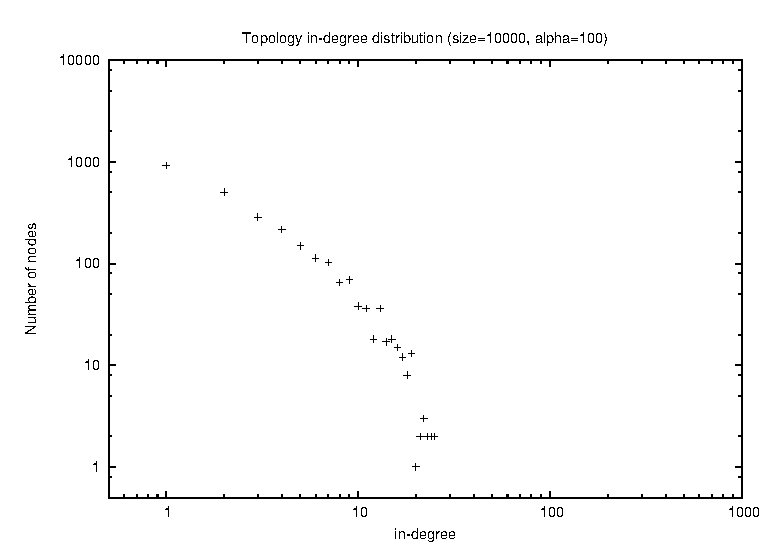
\includegraphics[scale=0.6]{picdegree_alfa100.eps}
\end{center}
\caption{In-degree distribution with $\alpha$ 100\label{d100figure}}
\end{figure}

\begin{figure}[tb!]
\begin{center}
\includegraphics[scale=0.6]{pic_alfa2000.eps}
\end{center}
\caption{Topology with $\alpha$ 2000\label{t2000figure}}
\end{figure}

\begin{figure}[tb!]
\begin{center}
\includegraphics[scale=0.6]{picdegree_alfa2000.eps}
\end{center}
\caption{In-degree distribution with $\alpha$ 2000\label{d2000figure}}
\end{figure}

\end{document}
